\chapter{Architectural Design}
\section{Overview}
This chapter focuses on the architectural structure, components will be described explaining how they interact with each other.
The system will be illustrated both physically and logically.\\
The main high level components of the system are the following:\\
\begin{itemize}
    \item
    \textbf{Applicaton device:} User's device where the application is installed. This application implements most of the logic of the system.
    \item
    \textbf{Cloud server:}  The server side of the system is responsible for the data storage and sync.\\ This layer contains a NoSQL database is used, 
    which stores data in flexible, JSON-like documents. The main keys are flexiblility, expressive querying, realtime updates, offline support and scalability.\\
    \item
    \textbf{Applicaton web:} A pre-existing application used by responsibles that allows to check and edit the stored data.
\end{itemize}
\clearpage
\section{Component View}
\subsection{High-Level Component View}
\begin{figure}[!h]
    \centering
    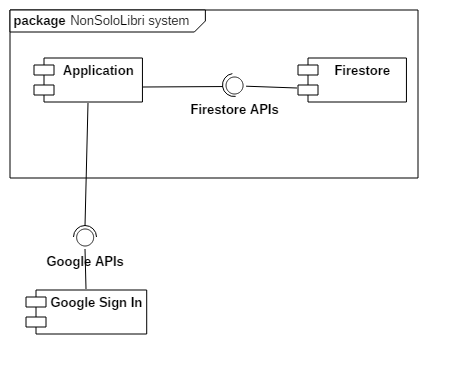
\includegraphics[scale=0.5]{images/high-level-component-view.png}
    \caption{High level component diagram}
    \label{ref:highlevelcomponentdiagram}
\end{figure}
This component diagram displays the high-level view of the sistem focusing on application device.
The component developed are:
\begin{itemize}
    \item
    \textbf{Application:} It is the core of the system, it manages all information provided by the others services
     and performs the majority of the functions. It provides the client access to the entire system.
    \item
    \textbf{Firestore:} This component has an account manager and backup roles. It receives the data from the application and provides them when necessary.
\end{itemize}
Moreover, application is integrated with \textbf{Google Sign In}, which provides the authatication functions of the system, 
using directly the credetial of Google.
\clearpage
\subsection{Application}
\begin{figure}[!h]
    \centering
    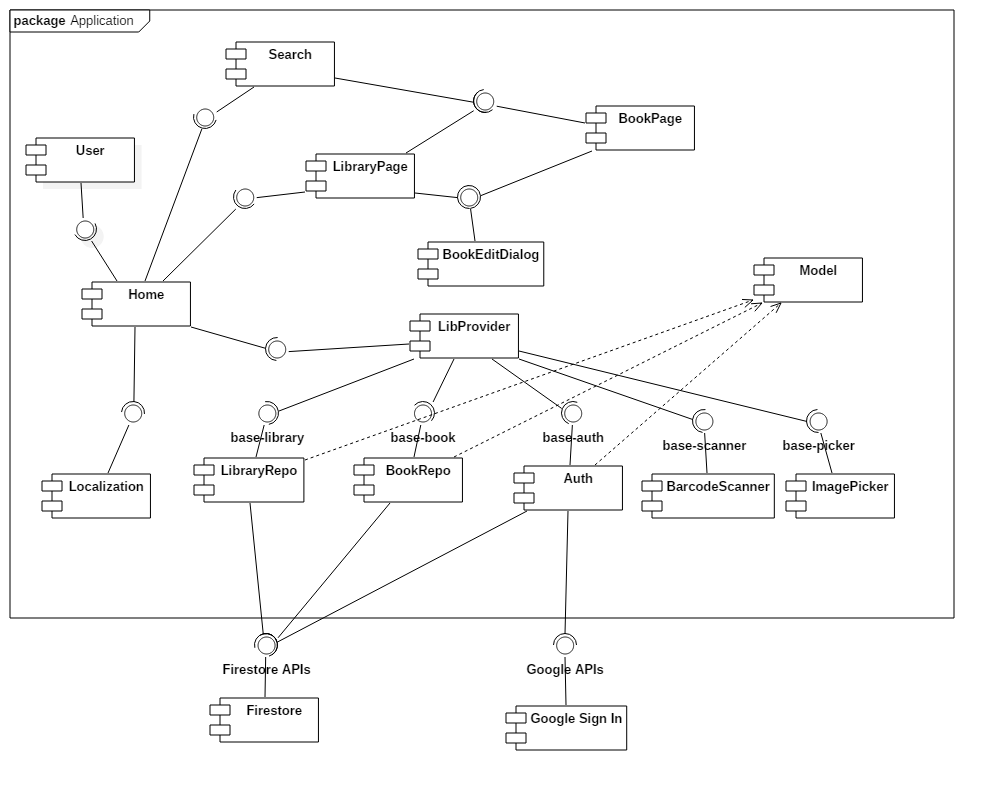
\includegraphics[scale=0.4]{images/application-component-diagram.png}
    \caption{Application component diagram}
    \label{ref:applicationcomponentdiagram}
\end{figure}
\begin{itemize}
    \item
    \textbf{Model:} It represents how the data are structured in the application and ready to be stored by Firestore.
    \item
    \textbf{Home:} Is is the entry point of the application. Creates the Localization and LibProvider components. Handles login parts and the choice of the library.
    \item
    \textbf{Localization:} It setups the language of the application based on the language of the OS.
    \item
    \textbf{LibProvider:} Provides LibraryRepo, BookRepo,Auth, BarcodeScanner and ImagePicker.
    \item
    \textbf{LibraryRepo:} This components is used to communicate with Firebase and to manage the library collection.
    \item
    \textbf{BookRepo:} It communicates with Firebase and saves an retrives the data of the book.
    \item
    \textbf{Auth:} This components is used to handle the authentication phase of the user.
    \item
    \textbf{BarcodeScanner:} It uses the camera the ISBN from the barcode of a book.
    \item
    \textbf{ImagePicker:} It uses the library that allows to take a photo with camera or pick an image from the gallery of the device.
    \item
    \textbf{LibraryPage:} It is the union of widgets that shows the books that belong to a given library.
    \item
    \textbf{BookPage:} It handles the infromation of the book, its reviews and the associated offers by the users. 
    \item
    \textbf{Search:} Shows a list of the books, which match with a user's input.
    \item
    \textbf{User:} It is the group of pages and widget that handles the profiles management, including friendships and conversation between users.
\end{itemize}
\clearpage
\section{Relationship between the model and the database}
During the design of the application has been used a database first approach. The database was the core during the design and the model was derived from it 
respecting the existing relationships between the entities.\\
The following there is the ER digram used to implements the database:
\begin{figure}[!h]
    \centering
    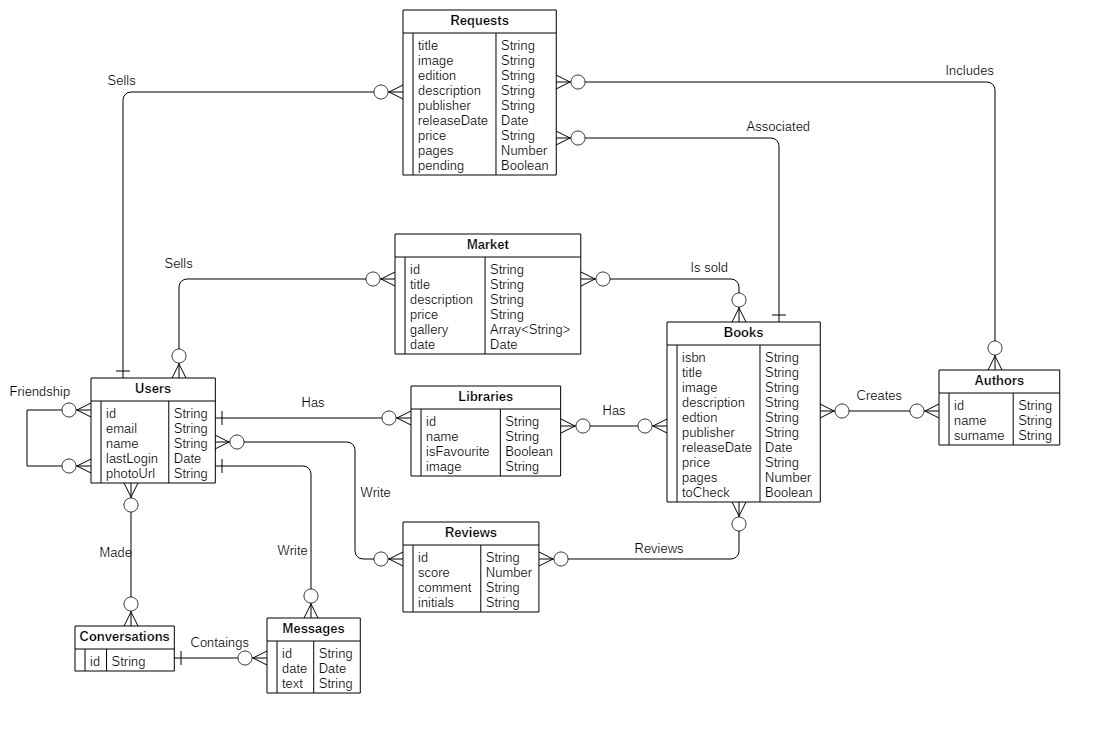
\includegraphics[scale=0.43]{images/er-diagram.png}
    \caption{ER diagram}
    \label{ref:erdiagram}
\end{figure}
\begin{itemize}
    \item
    \textbf{Books:} Collects all information of the books contained in the database. Each book is characterized  by a ISBN, which is its primary key, and other information including a title, a description and a image.
    \item
    \textbf{Users:} The users use the login function of the application. The id is generated automatically, the name and email are saved, but the password no.
    \item
    \textbf{Libraries:} The libraries created by each user.
    \item
    \textbf{Reviews:} Includes a score and a comment wrote by a user associated to a book.
    \item
    \textbf{Authors:} Contains the main of information of the creator of one or more books.
    \item
    \textbf{Requests:} Contains all suggestions made by a user to edit the book information. The idetifier is the union of the ISBN of the book and the user's id.
    \item
    \textbf{Market:} Collects the sales offers of books made by each user.
    \item
    \textbf{Conversations:} The discussion between two or more users.
    \item
    \textbf{Messages:} The texts exchanged during a conversation.
\end{itemize}
During the implementation, we have opted for the introduction of data duplication. This allows to yield the main characteristics of the document-oriented database.


